% Fig.: time of a ghost and of a restore against the simulated GitHub (report/data/measurements.json),
% and the lower bound GitHub's write pacing puts on the same operations.
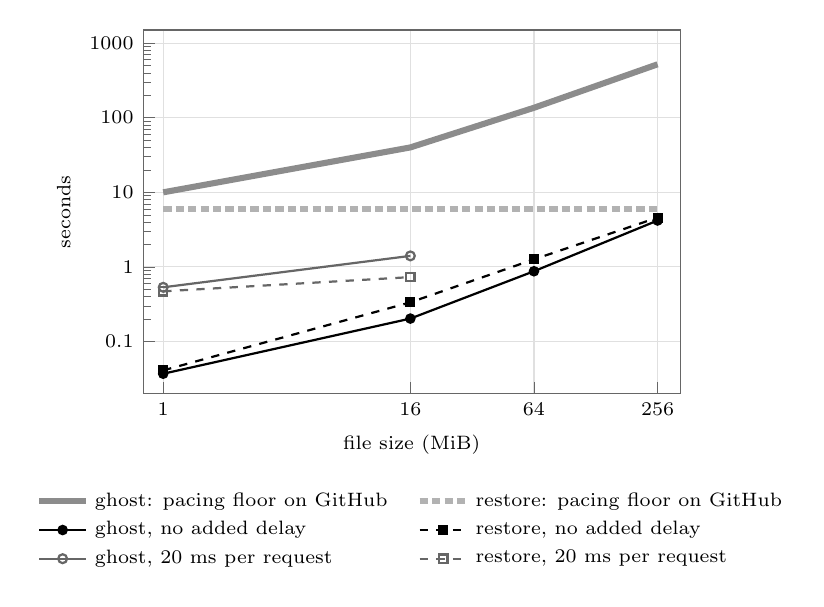
\begin{tikzpicture}
\begin{loglogaxis}[
  width=84mm, height=62mm,
  font=\scriptsize,
  xlabel={file size (MiB)}, ylabel={seconds},
  xmin=0.8, xmax=330, ymin=0.02, ymax=1500,
  xtick={1,16,64,256}, xticklabels={1,16,64,256},
  ytick={0.1,1,10,100,1000}, yticklabels={0.1,1,10,100,1000},
  grid=major, grid style={black!12},
  axis line style={black!60}, tick style={black!60},
  xtick pos=bottom, ytick pos=left,
  legend columns=2,
  legend style={font=\scriptsize, draw=none, at={(0.5,-0.24)}, anchor=north, cells={anchor=west},
                /tikz/every even column/.append style={column sep=3mm}},
  legend cell align=left,
  every axis plot/.append style={every mark/.append style={solid}},
]
\addplot[black!45, line width=2.2pt, mark=none] coordinates {(1,10) (16,40) (64,136) (256,520)};
\addlegendentry{ghost: pacing floor on GitHub}
\addplot[black!30, line width=2.2pt, mark=none, dash pattern=on 3pt off 1.5pt] coordinates {(1,6) (16,6) (64,6) (256,6)};
\addlegendentry{restore: pacing floor on GitHub}
\addplot[black, thick, mark=*, mark size=1.5pt] coordinates {(1,0.037) (16,0.203) (64,0.875) (256,4.189)};
\addlegendentry{ghost, no added delay}
\addplot[black, thick, mark=square*, mark size=1.4pt, dashed] coordinates {(1,0.041) (16,0.335) (64,1.263) (256,4.585)};
\addlegendentry{restore, no added delay}
\addplot[black!60, thick, mark=o, mark size=1.6pt] coordinates {(1,0.533) (16,1.406)};
\addlegendentry{ghost, 20 ms per request}
\addplot[black!60, thick, mark=square, mark size=1.5pt, dashed] coordinates {(1,0.471) (16,0.730)};
\addlegendentry{restore, 20 ms per request}
\end{loglogaxis}
\end{tikzpicture}
